%% bacon_cs.tex — Zurich Day 3 (morning): Bacon decomposition + Callaway-Sant'Anna
%% Scott Cunningham, University of Zurich, May 13, 2026
%%
%% Compile: pdflatex bacon_cs.tex
%% Style:   remix.sty (in same directory)
%%
%% Pedagogical arc (Scott's spec):
%%   1. Capture attention with a paper/problem/example
%%   2. Introduce the idea with data viz, beautiful tables, numerical examples
%%   3. TWFE = weighted average of 2x2s, algebraic OLS mechanics (Angrist 1998, Tymon 2022)
%%   4. Cross-check against Goodman-Bacon (2021) JoE original
%%   5. Step-by-step 2x2 -> ATT_k + PTB - DeltaATT_l derivation (the "forbidden comparison")
%%   6. Codeblock form of baker.do; visualize staggered structure
%%   Then: Callaway-Sant'Anna, linked to DR from the afternoon
%%
%% Running example: Stevenson-Wolfers (2006) no-fault divorce — the same data
%% Goodman-Bacon (2021) uses in his JoE paper.
%% Running simulation: baker.do — 4 cohorts, dynamic TE, truth = 82, TWFE = -6.69

\documentclass[aspectratio=169,11pt]{beamer}
\usepackage{remix}

\usepackage{tikz}
\usetikzlibrary{positioning,arrows.meta,calc,shapes.geometric,fit,backgrounds}
\usepackage{listings}
\usepackage{xcolor}
\usepackage{booktabs}
\usepackage{colortbl}
\usepackage{multirow}

% Cohort palette — extra colors for the four-cohort worksheets
\definecolor{gold}{HTML}{D69E2E}
\definecolor{harvardcrimson}{HTML}{A51C30}

% Stata language for listings (keywords without underscores to avoid lst-param errors)
\lstdefinelanguage{Stata}{
  morekeywords={areg, reg, regress, gen, generate, replace, by, bysort, drop, keep, sort,
                use, save, clear, set, seed, obs, expand, label, variable, egen, su, summarize,
                display, capture, log, close, exit, if, in, ssc, install, net, ivar, time,
                gvar, ipw, dripw, long2, csdid, drdid, xtdidregress, estat, bdecomp, ddtiming,
                group, calendar, event, simple, rnormal, runiform, cond},
  sensitive=true,
  morecomment=[l]{*},
  morecomment=[l]{//},
  morestring=[b]",
}

\lstset{
  basicstyle=\ttfamily\footnotesize,
  keywordstyle=\color{remixgreendark}\bfseries,
  commentstyle=\color{warmgray}\itshape,
  stringstyle=\color{ocean},
  backgroundcolor=\color{lightbg},
  frame=single,
  framesep=4pt,
  rulecolor=\color{warmgray!40},
  columns=fullflexible,
  showstringspaces=false,
  breaklines=true,
  numbers=none,
  xleftmargin=0.4em,
  xrightmargin=0.4em,
}

\renewcommand{\remixfooter}{University of Zurich\,\textperiodcentered\,Department of Economics\,\textperiodcentered\,May 2026}

\begin{document}

%% =====================================================================
%%                                ACT I
%% =====================================================================

%% ---------- Slide 1: TITLE ----------
\remixtitleframe
  {Staggered DiD: Bacon $+$ Callaway-Sant'Anna}
  {Day 3 of 3: Morning}
  {Scott Cunningham \textperiodcentered\ Baylor University}
  {University of Zurich \textperiodcentered\ May 13, 2026}

%% ---------- Slide 2: SW story ----------
\begin{frame}{Stevenson \&\ Wolfers (2006): can law reduce intimate violence?}
\vspace{0.4em}
Before 1969, divorce in the U.S.\ required showing fault --- adultery, abandonment, cruelty --- and either spouse could veto. \;Starting with California in 1969, states began adopting \highlight{unilateral divorce} laws: either spouse can dissolve the marriage, no fault required, no veto. \;By 1985 most states had moved.

\vspace{0.6em}
\textbf{The theory.} \;Lower exit cost shifts bargaining power within marriage. \;A woman with a credible threat to leave faces less violence and depression. \;Less violence, less depression $\Rightarrow$ fewer suicides.

\vspace{0.6em}
\textbf{The question.} \;Did the staggered timing of unilateral-divorce reforms reduce women's suicide rates?

\vspace{0.4em}
\meta{Stevenson, B., and J.\ Wolfers (2006). ``Bargaining in the Shadow of the Law: Divorce Laws and Family Distress.'' \textit{QJE} 121(1): 267--288.}
\end{frame}

%% ---------- Slide 3: SW data + design ----------
\begin{frame}{Their data and design}
\vspace{0.5em}
\textbf{Data.} \;NCHS Multiple Cause of Death (1964--1996); 1960 Census $+$ SEER for population denominators; SW's own coding of state divorce-law dates.

\vspace{0.4em}
\textbf{Outcome.} \;Age-adjusted female suicide rate per million women.

\vspace{0.4em}
\textbf{Sample.} \;37 states that adopted unilateral divorce 1969--1985 (staggered); 14 control states (5 never-reform, 8 pre-1964 reform, 1 excluded).

\vspace{0.6em}
\textbf{The design.} \;Staggered two-way fixed effects:
\begin{center}\small
$y_{ist} \;=\; \alpha_i \;+\; \gamma_t \;+\; \delta\, D_{ist} \;+\; \varepsilon_{ist}$
\end{center}

\vspace{0.4em}
\textbf{Their headline.} \;An 8--16\%\ decline in women's suicide rate in unilateral-divorce states, growing over time. \;Companion declines in domestic violence and intimate-partner homicide.
\end{frame}

%% ---------- Slide 4: The event study ----------
\begin{frame}{Their event study: the effect grows over time}
\begin{center}
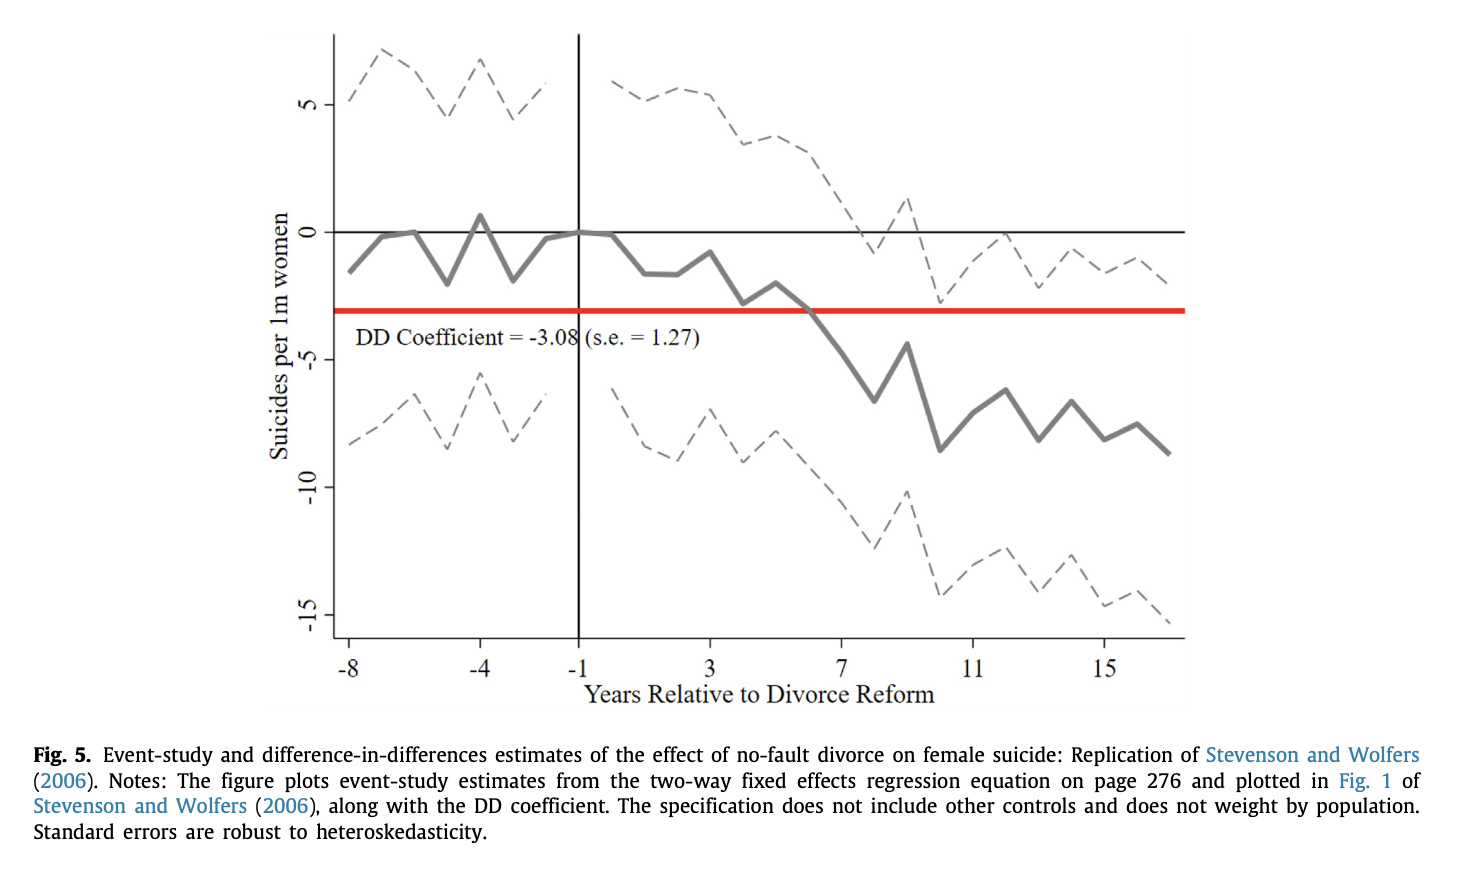
\includegraphics[width=0.68\textwidth,height=0.58\textheight,keepaspectratio]{figures/bacon_sw_eventstudy.png}
\end{center}
\vspace{-0.3em}
\begin{center}\small\color{warmgray}\itshape
Event study of no-fault divorce on female suicide (replication of SW from Bacon 2021, Fig.\ 5). \;Post-reform coefficients drift down to $\approx -10$ per million women. \;Red line: static TWFE returns \highlight{$-3.08$ (s.e.\ 1.27)} --- much smaller than the event-study average.
\end{center}
\end{frame}

%% ---------- Slide 5: Is the finding unbiased? ----------
\begin{frame}{Their finding $\;-3.08\;$ (s.e.\ 1.27).  Is it unbiased?}
\begin{center}

\includegraphics[width=0.78\textwidth,height=0.62\textheight,keepaspectratio]{figures/bacon_sw_sampling_dist.pdf}
\end{center}
\vspace{-0.3em}
\begin{center}\small\color{warmgray}\itshape
$\widehat{\beta}^{\text{TWFE}}$ converges to its OLS population estimand at $-3.08$ (LLN/CLT). \;That much is unbiased.
\;Whether the estimand IS the ATT is a \textit{separate} question --- and under heterogeneity, the bias is $-\Delta\text{ATT}$, somewhere we cannot pin down without more structure.
\end{center}
\end{frame}

%% ---------- Slide 6: Bacon decomposes the estimand ----------
\begin{frame}{What \textit{is} the estimand?  Bacon decomposes it into 156 components}
\vspace{0.5em}
Bacon (2021) writes the TWFE estimand as a weighted average of underlying 2$\times$2 DiDs. \;On SW data: 156 components.

\vspace{0.7em}
\begin{itemize}
  \item Late-treated-vs-already-treated 2$\times$2s average \highlight{$+3.51$} --- the \textit{wrong sign}, pulled there by treatment-effect heterogeneity over time.
  \vspace{0.3em}
  \item Drop those terms: the rest averages $-5.44$, very close to the event-study average of $-4.92$ from the figure two slides back.
\end{itemize}

\vspace{0.7em}
\textbf{So the estimand $-3.08$ is averaging $+3.51$ with $-5.44$.} \;Both pieces come from the same regression on the same data. \;\highlight{Whether either piece is the ATT depends on what we assume.}

\vspace{0.4em}
That's what this morning develops.
\meta{Goodman-Bacon, A.\ (2021), \textit{J.\ Econometrics} 225(2): 254--277. \;Decomposition in Fig.\ 6.}
\end{frame}

%% ---------- Slide 4: Roadmap ----------
\begin{frame}{This morning, two acts}
\vspace{0.4em}
\begin{enumerate}
  \item \textbf{Why TWFE goes wrong (Goodman-Bacon 2021).} \;TWFE is a variance-weighted average of every 2$\times$2 DiD in the data. \;Some of those 2$\times$2s use \textit{already-treated} units as controls. \;When effects are dynamic, that's poison.
  \vspace{0.3em}
  \item \textbf{Callaway \& Sant'Anna (2021), the fix.} \;Forward-engineer from the target parameter $\text{ATT}(g,t)$. \;Estimate each one with the never-treated or not-yet-treated --- never the already-treated. \;Then aggregate.
\end{enumerate}

\vspace{0.6em}
\begin{center}
\small\color{warmgray}\itshape
The afternoon-morning thread: yesterday's DR-DiD is the engine inside CS's ATT(g,t).
\end{center}
\end{frame}

%% =====================================================================
%%                                LESSON 1
%% =====================================================================
\remixsection{1.\ Bacon's decomposition \\[0.3em] {\normalsize\normalfont TWFE is a weighted average of 2$\times$2 DiDs --- and OLS picks the weights}}

%% ---------- L1-F1: The claim ----------
\begin{frame}{Bacon's claim: TWFE \textit{is} a weighted average of 2$\times$2s}
\vspace{0.4em}
The TWFE regression with $K$ timing groups produces an estimate $\widehat{\delta}^{\text{TWFE}}$ that is \textit{numerically identical} to a weighted average of every 2$\times$2 DiD you can construct from the data.
\vspace{0.6em}

\begin{block}{The decomposition (informally)}
\centering
$\widehat{\delta}^{\text{TWFE}} \;=\; \displaystyle\sum_{\text{every 2}\times\text{2 in the data}} s_{ij}\, \widehat{\delta}^{2\times 2}_{ij}$
\end{block}

\vspace{0.6em}
\begin{itemize}\small
  \item This is \textit{pure} OLS algebra. \;No assumptions about treatment effects yet.
  \item It's also not surprising: any OLS coefficient is a weighted average of some underlying ``comparison'' --- Angrist (1998), Tymon (2022) for the general result.
  \item The interesting questions: \;\highlight{which 2$\times$2s, with what weights, and is the average we get the average we want?}
\end{itemize}
\end{frame}

%% ---------- L1-F2: The K^2 distinct DDs ----------
\begin{frame}{With $K$ timing groups, there are many 2$\times$2s}
\vspace{0.4em}
Three timing groups $\{a, b, c\}$ plus one never-treated group $U$. \;Bacon counts the 2$\times$2s:

\vspace{0.6em}
\begin{center}
\begin{tabular}{ccc}
\toprule
\textbf{Treated vs.\ Never} & \textbf{Treated vs.\ Later} & \textbf{Treated vs.\ Earlier} \\
\midrule
$a$ vs.\ $U$ & $a$ vs.\ $b$ \;(later) & $b$ vs.\ $a$ \;(earlier) \\
$b$ vs.\ $U$ & $a$ vs.\ $c$ \;(later) & $c$ vs.\ $a$ \;(earlier) \\
$c$ vs.\ $U$ & $b$ vs.\ $c$ \;(later) & $c$ vs.\ $b$ \;(earlier) \\
\bottomrule
\end{tabular}
\end{center}

\vspace{0.7em}
\begin{itemize}\small
  \item Column 1: the comparisons you intended.
  \item Column 2: still uses an \textit{eventually}-treated unit as a control --- it's fine, because that unit hasn't been treated yet in the comparison window.
  \item Column 3: uses an \textit{already}-treated unit as a control. \;\highlight{This is the forbidden comparison.}
\end{itemize}
\end{frame}

%% ---------- L1-F3: The two flavors of 2x2 between timing groups ----------
\begin{frame}{Two timing groups: $k$ (early) and $\ell$ (late)}
\vspace{0.4em}
Three time windows: \;\textsc{Pre}, \;\textsc{Mid}\;\;(between the two treatment dates), \;\textsc{Post}.

\vspace{0.6em}
\begin{itemize}\small
  \item \textbf{$k$ vs.\ $\ell$ during \textsc{Mid}.} \;Group $k$ is post-treatment; group $\ell$ is still pre-treatment. \;\highlight{Comparison is fine} --- $\ell$ is a not-yet-treated control.
\end{itemize}
\vspace{0.3em}
\begin{center}\small
$\widehat{\delta}_{k\ell}^{2\times 2,\,k} \;=\; \big(\bar y_k^{\textsc{Mid}} - \bar y_k^{\textsc{Pre}}\big) \;-\; \big(\bar y_\ell^{\textsc{Mid}} - \bar y_\ell^{\textsc{Pre}}\big)$
\end{center}

\vspace{0.7em}
\begin{itemize}\small
  \item \textbf{$\ell$ vs.\ $k$ during \textsc{Post}.} \;Group $\ell$ is post-treatment; group $k$ is \textit{also} post-treatment. \;\highlight{The forbidden comparison} --- $k$ is now an already-treated control.
\end{itemize}
\vspace{0.3em}
\begin{center}\small
$\widehat{\delta}_{\ell k}^{2\times 2,\,\ell} \;=\; \big(\bar y_\ell^{\textsc{Post}} - \bar y_\ell^{\textsc{Mid}}\big) \;-\; \big(\bar y_k^{\textsc{Post}} - \bar y_k^{\textsc{Mid}}\big)$
\end{center}
\end{frame}

%% ---------- L1-F3b: The forbidden 2x2 visualized ----------
\begin{frame}{The forbidden 2$\times$2, visualized}
\begin{center}
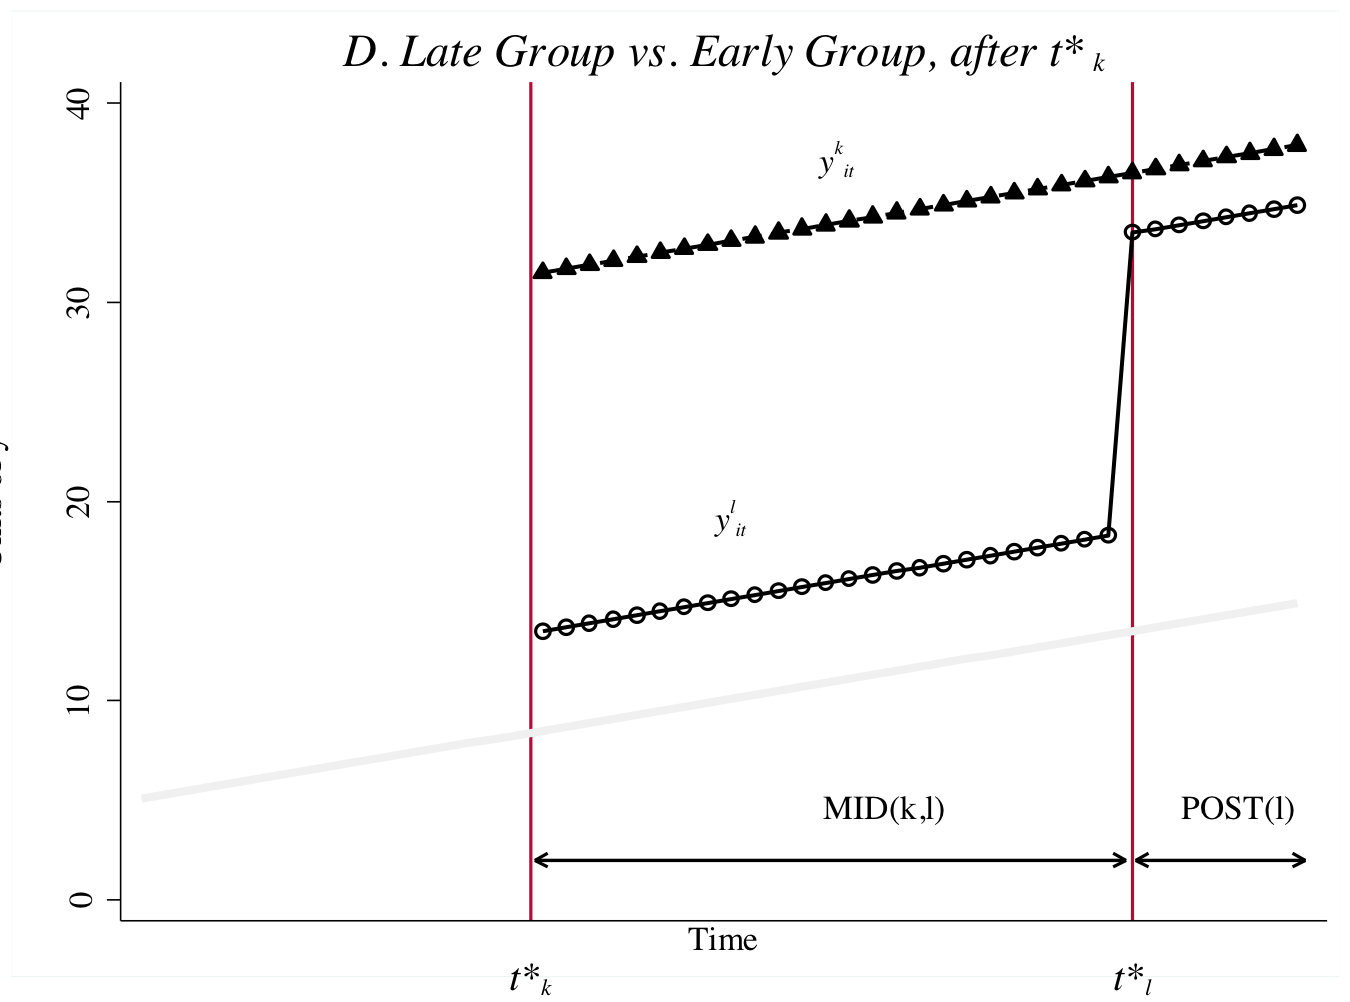
\includegraphics[width=0.78\textwidth,height=0.7\textheight,keepaspectratio]{figures/bacon_forbidden_2x2.png}
\end{center}
\vspace{-0.2em}
\begin{center}
\small\color{warmgray}\itshape
Group $\ell$ treated in \textsc{Post}; group $k$ \textit{already treated} since \textsc{Mid}. \;One side is a treated unit that should never have been a control.
\end{center}
\end{frame}

%% ---------- L1-F4: Bacon's decomposition formally ----------
\begin{frame}{The full Bacon decomposition}
\vspace{0.4em}
\textbf{The setup.} $K$ timing groups, possibly one never-treated group $U$. \;TWFE estimate:

\vspace{0.2em}
\[
\widehat{\delta}^{\text{TWFE}} \;=\; \underbrace{\sum_{k\neq U} s_{kU}\, \widehat{\delta}^{2\times 2}_{kU}}_{\text{treated vs.\ never-treated}} \;+\; \underbrace{\sum_{k\neq U}\sum_{\ell > k} s_{k\ell}\!\left[ \mu_{k\ell}\, \widehat{\delta}^{2\times 2,\,k}_{k\ell} \;+\; (1-\mu_{k\ell})\, \widehat{\delta}^{2\times 2,\,\ell}_{\ell k}\right]}_{\text{treated vs.\ another-timing-group}}
\]

\vspace{0.5em}
\begin{itemize}\small
  \item First sum: every timing group compared to the never-treated. Clean.
  \item Second sum: every \textit{pair} of timing groups $(k, \ell)$ with $k$ earlier, $\ell$ later, contributes two 2$\times$2s --- one with $\ell$ as not-yet-treated control (fine), one with $k$ as already-treated control (\highlight{forbidden}).
  \item Weights $s_{kU}, s_{k\ell}$, and the within-pair weight $\mu_{k\ell}$ come from OLS algebra, not theory.
\end{itemize}
\meta{Notation: we write the forbidden 2$\times$2 as $\widehat{\delta}^{2\times 2,\ell}_{\ell k}$. Bacon (2021, Eq.\ 10a) writes it as $\widehat{\beta}^{2\times 2,\ell}_{k\ell}$. Same object; we follow Scott's CI-2 convention.}
\end{frame}

%% ---------- L1-F5: The variance weights ----------
\begin{frame}{Where the weights come from: variance of $\tilde D$}
After de-meaning $D_{it}$ within unit and time, what remains is $\tilde D_{it}$. \;The Bacon weights are functions of $\widehat{\mathrm{Var}}(\tilde D_{it})$ and group shares:
\begin{align*}
s_{kU} &\;=\; \frac{n_k\, n_U\, \overline{D}_k(1-\overline{D}_k)}{\widehat{\mathrm{Var}}(\tilde D_{it})} \\[0.2em]
s_{k\ell} &\;=\; \frac{n_k\, n_\ell\, (\overline{D}_k - \overline{D}_\ell)\big(1 - (\overline{D}_k - \overline{D}_\ell)\big)}{\widehat{\mathrm{Var}}(\tilde D_{it})} \\[0.2em]
\mu_{k\ell} &\;=\; \frac{1 - \overline{D}_k}{1 - (\overline{D}_k - \overline{D}_\ell)}
\end{align*}
\begin{itemize}\small
  \item $\overline{D}_k$ is the share of group $k$'s panel spent in treatment.
  \item Same variance-weighting Angrist (1998) and Tymon (2022) describe generally: OLS weights treatment contrasts by treatment-status variance.
\end{itemize}
\end{frame}

%% ---------- L1-F6: Weight intuition ----------
\begin{frame}{Variance is maximized in the middle of the panel}
\vspace{0.4em}
Consider the never-treated 2$\times$2 weight, $s_{kU}$. \;The key factor: $\overline{D}_k(1-\overline{D}_k)$.

\vspace{0.6em}
\begin{center}
\begin{tabular}{cc}
\toprule
$\overline{D}_k$ \;\;(share of panel treated) & $\overline{D}_k(1-\overline{D}_k)$ \\
\midrule
$0.1$ & $0.09$ \\
$0.3$ & $0.21$ \\
$0.5$ & $\mathbf{0.25}$ \;\;\highlight{$\leftarrow$ max} \\
$0.7$ & $0.21$ \\
$0.9$ & $0.09$ \\
\bottomrule
\end{tabular}
\end{center}

\vspace{0.7em}
\begin{itemize}\small
  \item Groups treated in the \textit{middle} of the panel get the highest weight.
  \item Same logic for $(\overline{D}_k - \overline{D}_\ell)\big(1 - (\overline{D}_k - \overline{D}_\ell)\big)$.
  \item \highlight{Panel length affects the weights.} \;Trim the panel and you've changed the estimand.
\end{itemize}
\end{frame}

%% ---------- L1-F7: bridge to potential outcomes ----------
\begin{frame}{So far: pure algebra. Now: potential outcomes.}
\vspace{0.5em}
What we have:
\begin{itemize}\small
  \item TWFE is a weighted average of 2$\times$2s.
  \item Some of those 2$\times$2s use already-treated units as controls.
  \item OLS picks the weights based on treatment variance.
\end{itemize}

\vspace{0.5em}
What we don't yet have:
\begin{itemize}\small
  \item Whether the weighted average we get \textit{is} the weighted ATT we want.
\end{itemize}

\vspace{0.6em}
\highlight{To answer that we need to switch from realized outcomes to potential outcomes.}

\vspace{0.5em}
\begin{center}
\small\color{warmgray}\itshape
The next four slides walk through a single 2$\times$2 step by step, then substitute back into the decomposition. The result is a clean expression for the bias.
\end{center}
\end{frame}

%% =====================================================================
%%                                LESSON 2
%% =====================================================================
\remixsection{2.\ The forbidden 2$\times$2, step by step \\[0.3em] {\normalsize\normalfont Add a zero, rearrange, and the bias appears}}

%% ---------- L2-F1: Step 1 — the 2x2 in observed outcomes ----------
\begin{frame}{Step 1 --- write down the 2$\times$2 in observed outcomes}
\vspace{0.4em}
The 2$\times$2 we're worried about: group $\ell$ (later-treated) in \textsc{Post}, with group $k$ (earlier-treated) as control.

\vspace{0.6em}
\begin{center}
\fbox{\parbox{0.92\textwidth}{
\centering
\vspace{0.2em}
$\widehat{\delta}^{2\times 2,\,\ell}_{\ell k} \;=\; \big[\bar y_\ell^{\textsc{Post}} \;-\; \bar y_\ell^{\textsc{Mid}}\big] \;-\; \big[\bar y_k^{\textsc{Post}} \;-\; \bar y_k^{\textsc{Mid}}\big]$
\vspace{0.2em}
}}
\end{center}

\vspace{0.7em}
\begin{itemize}\small
  \item Both groups are \textit{treated} in \textsc{Post}.
  \item Both groups were \textit{treated} in \textsc{Mid}? \;No --- $\ell$ is still untreated in \textsc{Mid}.
  \item So group $\ell$'s ``change'' includes its move from untreated to treated. Group $k$'s ``change'' is from \textit{treated} to \textit{treated}.
\end{itemize}
\end{frame}

%% ---------- L2-F2: Step 2 — substitute potential outcomes ----------
\begin{frame}{Step 2 --- switch to potential outcomes}
\vspace{0.4em}
Replace each observed mean with the appropriate potential-outcome mean (using the switching equation):

\vspace{0.4em}
\begin{align*}
\bar y_\ell^{\textsc{Post}} &\;=\; \mathbb{E}[Y^1 \mid \ell, \textsc{Post}] \quad &\text{(treated)} \\
\bar y_\ell^{\textsc{Mid}}  &\;=\; \mathbb{E}[Y^0 \mid \ell, \textsc{Mid}]   \quad &\text{(not yet treated)} \\
\bar y_k^{\textsc{Post}}    &\;=\; \mathbb{E}[Y^1 \mid k, \textsc{Post}]    \quad &\text{(treated)} \\
\bar y_k^{\textsc{Mid}}     &\;=\; \mathbb{E}[Y^1 \mid k, \textsc{Mid}]     \quad &\text{(already treated)}
\end{align*}

\vspace{0.3em}
\highlight{Notice the asymmetry.} \;Group $k$ is in $Y^1$ in \textit{both} \textsc{Mid} and \textsc{Post}. \;That's the problem.

\vspace{0.5em}
\begin{center}
\small\color{warmgray}\itshape
Three of the four cells are $Y^1$. Only one is $Y^0$.
\end{center}
\end{frame}

%% ---------- L2-F3: Step 3 — add zeros ----------
\begin{frame}{Step 3 --- add zeros}
\vspace{0.4em}
We add three zero-valued terms of the form $\mathbb{E}[Y^0 \mid \cdot] - \mathbb{E}[Y^0 \mid \cdot]$:

\vspace{0.4em}
\begin{block}{The three zeros}
\small
\begin{enumerate}
  \item $+\mathbb{E}[Y^0 \mid \ell, \textsc{Post}] - \mathbb{E}[Y^0 \mid \ell, \textsc{Post}]$ \quad (add to $\ell$ in \textsc{Post})
  \item $+\mathbb{E}[Y^0 \mid k, \textsc{Post}] - \mathbb{E}[Y^0 \mid k, \textsc{Post}]$ \quad (add to $k$ in \textsc{Post})
  \item $+\mathbb{E}[Y^0 \mid k, \textsc{Mid}]  - \mathbb{E}[Y^0 \mid k, \textsc{Mid}]$  \quad (add to $k$ in \textsc{Mid})
\end{enumerate}
\end{block}

\vspace{0.5em}
\begin{itemize}\small
  \item Each adds zero. \;The 2$\times$2 is unchanged.
  \item But now we can group the terms into something interpretable.
\end{itemize}
\end{frame}

%% ---------- L2-F4: Step 4 — rearrange ----------
\begin{frame}{Step 4 --- rearrange into ATT, parallel-trends, and $\Delta$ATT}
\vspace{0.3em}
Group the eight terms (four observed $+$ four added zeros) into three buckets:
\vspace{0.4em}

\begin{block}{The forbidden 2$\times$2 in causal pieces}
\small
\centering
$\widehat{\delta}^{2\times 2,\,\ell}_{\ell k} \;=\; \underbrace{\text{ATT}_\ell(\textsc{Post})}_{\text{what we want}} \;+\; \underbrace{\Delta Y^0_\ell(\textsc{Post},\textsc{Mid}) \;-\; \Delta Y^0_k(\textsc{Post},\textsc{Mid})}_{\text{parallel-trends bias}} \;-\; \underbrace{\big[\text{ATT}_k(\textsc{Post}) - \text{ATT}_k(\textsc{Mid})\big]}_{\text{heterogeneity bias: }\Delta\text{ATT}_k}$
\end{block}

\vspace{0.6em}
\begin{itemize}\small
  \item Bucket 1 is the ATT we want for group $\ell$ in the post-period.
  \item Bucket 2 is the standard PT bias --- requires PT between $\ell$ and $k$ in this window.
  \item Bucket 3 is \highlight{new}: it's the \textit{change} in group $k$'s own ATT between \textsc{Mid} and \textsc{Post}. \;If treatment effects grow (dynamics), this is positive --- and it enters with a \textit{minus sign}.
\end{itemize}
\end{frame}

%% ---------- L2-F5: Step 5 — substitute back, the decomposition ----------
\begin{frame}{Step 5 --- substitute back into Bacon's decomposition}
\vspace{0.4em}
The three flavors of 2$\times$2 in causal pieces:

\vspace{0.3em}
\begin{align*}
\widehat{\delta}^{2\times 2}_{kU} \;&=\; \text{ATT}_k(\textsc{Post}) \;+\; \Delta Y^0_k(\text{post},\text{pre}) - \Delta Y^0_U(\text{post},\text{pre}) \\[0.2em]
\widehat{\delta}^{2\times 2,\,k}_{k\ell} \;&=\; \text{ATT}_k(\textsc{Mid}) \;+\; \Delta Y^0_k(\textsc{Mid},\text{pre}) - \Delta Y^0_\ell(\textsc{Mid},\text{pre}) \\[0.2em]
\widehat{\delta}^{2\times 2,\,\ell}_{\ell k} \;&=\; \text{ATT}_\ell(\textsc{Post}) \;+\; \Delta Y^0_\ell(\textsc{Post},\textsc{Mid}) - \Delta Y^0_k(\textsc{Post},\textsc{Mid}) \\
                                          &\phantom{\;=\;}\; -\; \Delta\text{ATT}_k
\end{align*}

Plug these into Bacon's weighted sum. \;The TWFE probability limit:
\begin{center}
\highlight{$\text{plim}\, \widehat{\delta}^{\text{TWFE}} \;=\; \text{VWATT} \;+\; \text{VWPT} \;-\; \Delta\text{ATT}$}
\end{center}
\meta{Bacon (2021, Eq.\ 15) writes VWCT (variance-weighted \textit{common} trends). Same object as our VWPT.}
\end{frame}

%% ---------- L2-F6: Reading the result ----------
\begin{frame}{What the decomposition tells us}
\vspace{0.5em}
$\text{plim}\, \widehat{\delta}^{\text{TWFE}} \;=\; \text{VWATT} \;+\; \text{VWPT} \;-\; \Delta\text{ATT}$

\vspace{0.7em}
\begin{itemize}
  \item \textbf{VWATT} --- a variance-weighted ATT. \;Not the ATT \textit{you} want unless you specifically wanted variance-weighted averaging. \;The weights depend on \textit{panel length} (a researcher choice).
  \vspace{0.2em}
  \item \textbf{VWPT} --- variance-weighted parallel-trends bias. \;Zero only if PT holds across \textit{every} pairwise comparison, including between treated groups.
  \vspace{0.2em}
  \item \textbf{$\Delta$ATT} --- the dynamics term. \;If ATT grows with time-since-treatment, this is \textit{positive} and enters with a \textit{minus sign} --- attenuating TWFE toward zero, or even \highlight{flipping the sign}.
\end{itemize}

\vspace{0.6em}
\begin{center}
\small\color{warmgray}\itshape
That's exactly what happens in baker.do: dynamics big enough that $-\Delta\text{ATT}$ swamps the rest, flipping $+82$ to $-6.69$.
\end{center}
\end{frame}

%% =====================================================================
%%                                LESSON 3
%% =====================================================================
\remixsection{3.\ baker.do, in code \\[0.3em] {\normalsize\normalfont Set the seed, write the DGP, compute the truth, run TWFE, watch it fail}}

%% ---------- L3-F1a: The panel — the explicit-line discipline ----------
\begin{frame}[fragile]{The panel: 30 explicit lines, because repetition \textit{is} the lesson}
\begin{lstlisting}[basicstyle=\ttfamily\tiny]
set obs 40
gen state = _n
expand 25
bysort state: gen firms = runiform(0,5)
expand 30
sort state
bysort state firms: gen year = _n

replace year = 1980 if year==1
replace year = 1981 if year==2
replace year = 1982 if year==3
replace year = 1983 if year==4
replace year = 1984 if year==5
replace year = 1985 if year==6
replace year = 1986 if year==7   // cohort 1 first treated here
replace year = 1987 if year==8
replace year = 1988 if year==9
... (22 more explicit lines, one per year, through 2009) ...
\end{lstlisting}
\meta{A loop would be shorter. The 30 lines \textit{are the lesson}: each is one substitution, one beat. See \texttt{simulations/README.md} \S1.}
\end{frame}

%% ---------- L3-F1b: The DGP ----------
\begin{frame}[fragile]{The DGP, in 12 more explicit lines}
\begin{lstlisting}[language=Stata,basicstyle=\ttfamily\scriptsize]
set seed 20200403

* Group-specific TE means (heterogeneous across cohorts)
gen te1 = rnormal(10, 0.04)    // cohort 1986
gen te2 = rnormal( 8, 0.04)    // cohort 1992
gen te3 = rnormal( 6, 0.04)    // cohort 1998
gen te4 = rnormal( 4, 0.04)    // cohort 2004
gen te  = cond(group==1, te1, cond(group==2, te2, cond(group==3, te3, te4)))

* Y(0) and Y(1) under DYNAMIC effects (te grows since treatment)
gen y0         = firms + n + e
gen te_dynamic = te*treat*(year - treat_date + 1)
gen y          = y0 + te_dynamic
\end{lstlisting}
\meta{One step per line, named variables, no loops. \;Full file: \texttt{simulations/staggered/baker.do}.}
\end{frame}

%% ---------- L3-F2: The truth ----------
\begin{frame}[fragile]{The truth, computed before running anything}
\vspace{0.3em}
\begin{lstlisting}[language=Stata,basicstyle=\ttfamily\scriptsize]
* The truth (averaged across cohorts and post-periods)
su te_dynamic if treat == 1
display "True average ATT (dynamic) = " r(mean)
\end{lstlisting}

\vspace{0.6em}
Output: \;\highlight{\texttt{True average ATT (dynamic) $=$ 82}}

\vspace{0.8em}
\textbf{Why 82?} \;The dynamic effect for group 1 averages $(10 + 20 + \cdots + 240)/24$. \;Combined across cohorts and post-periods, the simple average is 82.

\vspace{0.5em}
\begin{center}
\small\color{warmgray}\itshape
We computed the truth from the DGP. \;Now compare it to what TWFE produces.
\end{center}
\end{frame}

%% ---------- L3-F3: TWFE result ----------
\begin{frame}[fragile]{TWFE, applied}
\begin{lstlisting}[language=Stata,basicstyle=\ttfamily\scriptsize]
areg y i.year treat, a(id) robust
\end{lstlisting}

\vspace{0.8em}
\begin{center}\large
\begin{tabular}{lcc}
\toprule
& \textbf{Truth} & \textbf{TWFE} \\
\midrule
$\widehat{\text{ATT}}$ & $+82$ & $-6.69^{\ast\ast\ast}$ \\
\bottomrule
\end{tabular}
\end{center}

\vspace{1em}
\highlight{Sign-flipped.} \;Extreme dynamics --- the $-\Delta\text{ATT}$ term swamps VWATT.
\end{frame}

%% ---------- L3-F4: Bacon decomposition table ----------
\begin{frame}{The Bacon decomposition of that $-6.69$}
\vspace{0.6em}
\begin{center}
\begin{tabular}{lcc}
\toprule
\textbf{DD comparison} & \textbf{Weight} & \textbf{Avg DD estimate} \\
\midrule
Earlier-treated vs.\ later-treated-(as-control) & $0.500$ & $+51.80$ \\
Later-treated vs.\ earlier-treated-(as-control) & $0.500$ & $-65.18$ \\
\bottomrule
\end{tabular}
\end{center}

\vspace{0.7em}
\begin{center}\large
$(0.5)(+51.80) \;+\; (0.5)(-65.18) \;=\; -6.69.$
\end{center}

\vspace{0.7em}
\textbf{Read it.} \;Half the weight is on a 2$\times$2 averaging $-65$ --- a 2$\times$2 that uses an already-treated group as control. \;\highlight{That's the forbidden comparison doing the damage.}
\end{frame}

%% =====================================================================
%%                                LESSON 4
%% =====================================================================
\remixsection{4.\ Visualizing staggered structure \\[0.3em] {\normalsize\normalfont What the cells look like, what TWFE averages over}}

%% ---------- L4-F1: The constant-TE grid ----------
\begin{frame}{Constant-TE worksheet}
\begin{center}\footnotesize
\begin{tabular}{c|cccc}
\toprule
\textbf{Year} & \textbf{ATT(1986,t)} & \textbf{ATT(1992,t)} & \textbf{ATT(1998,t)} & \textbf{ATT(2004,t)} \\
\midrule
1980--1985 & 0 & 0 & 0 & 0 \\
1986--1991 & \cellcolor{forest!18}10 & 0 & 0 & 0 \\
1992--1997 & \cellcolor{forest!18}10 & \cellcolor{ocean!22}8 & 0 & 0 \\
1998--2003 & \cellcolor{forest!18}10 & \cellcolor{ocean!22}8 & \cellcolor{gold!28}6 & 0 \\
2004--2009 & \cellcolor{forest!18}10 & \cellcolor{ocean!22}8 & \cellcolor{gold!28}6 & \cellcolor{harvardcrimson!18}4 \\
\midrule
ATT$(g)$ & 10 & 8 & 6 & 4 \\
\bottomrule
\end{tabular}
\end{center}

\vspace{0.4em}
\begin{itemize}\small
  \item \textbf{Simple ATT} (uniform avg over colored cells) $= 8.0$.
  \item \textbf{VWATT} (TWFE's target) $\neq 8.0$ --- OLS weights down edge cohorts via $\overline{D}(1-\overline{D})$.
\end{itemize}
\meta{Even with \textit{constant} effects per cohort, TWFE doesn't give the simple ATT.}
\end{frame}

%% ---------- L4-F2: The dynamic-TE grid ----------
\begin{frame}{Dynamic-TE worksheet}
\begin{center}\footnotesize
\begin{tabular}{c|cccc}
\toprule
\textbf{Year} & \textbf{ATT(1986,t)} & \textbf{ATT(1992,t)} & \textbf{ATT(1998,t)} & \textbf{ATT(2004,t)} \\
\midrule
1986 & \cellcolor{forest!18}10 & 0 & 0 & 0 \\
1992 & \cellcolor{forest!18}70 & \cellcolor{ocean!22}8 & 0 & 0 \\
1998 & \cellcolor{forest!18}130 & \cellcolor{ocean!22}56 & \cellcolor{gold!28}6 & 0 \\
2004 & \cellcolor{forest!18}190 & \cellcolor{ocean!22}104 & \cellcolor{gold!28}42 & \cellcolor{harvardcrimson!18}4 \\
2009 & \cellcolor{forest!18}240 & \cellcolor{ocean!22}144 & \cellcolor{gold!28}72 & \cellcolor{harvardcrimson!18}24 \\
\bottomrule
\end{tabular}
\end{center}

\vspace{0.5em}
ATT grows each year since treatment (the dynamic DGP). \;Simple ATT (uniform avg over colored cells) $\approx 82$; \;TWFE $= -6.69$.

\vspace{0.4em}
\highlight{The $-\Delta$ATT bias is doing the damage.} \;Late cohorts use the already-treated earlier cohorts as ``controls'' --- whose outcomes are growing.
\end{frame}

%% =====================================================================
%%                                LESSON 5
%% =====================================================================
\remixsection{5.\ Callaway \& Sant'Anna \\[0.3em] {\normalsize\normalfont Forward-engineer from ATT$(g,t)$, never use the already-treated as control}}

%% ---------- L5-F1: Forward engineering ----------
\begin{frame}{The forward-engineering principle}
\vspace{0.5em}
Bacon told us what reverse-engineering from TWFE buys you: \;a variance-weighted average of every 2$\times$2 in the data, including the forbidden ones.

\vspace{0.6em}
\textbf{The Callaway-Sant'Anna (2021) inversion:}
\begin{enumerate}\small
  \item \textbf{Start} with the target parameter you actually want: $\text{ATT}(g, t)$ --- the average treatment effect on cohort $g$ in calendar period $t$.
  \item \textbf{State} the identification assumptions formally.
  \item \textbf{Derive} an estimator directly from those assumptions.
  \item \textbf{Aggregate} the building blocks into whatever summary you want.
\end{enumerate}

\vspace{0.6em}
\begin{center}
\small\color{warmgray}\itshape
Each ATT$(g,t)$ is its own clean 2$\times$2 problem. \;Yesterday afternoon's DR-DiD is exactly the engine that estimates one.
\end{center}
\end{frame}

%% ---------- L5-F2: ATT(g,t) ----------
\begin{frame}{ATT$(g,t)$ --- the building block}
\vspace{0.6em}
\begin{block}{Definition}
\centering
$\text{ATT}(g, t) \;=\; \mathbb{E}\big[\, Y_{i,t}(1) - Y_{i,t}(0) \,\big|\, G_i = g\,\big]$
\end{block}

\vspace{0.6em}
\begin{itemize}\small
  \item $G_i = g$ \;$=$\; ``unit $i$ was first treated in period $g$.'' \;(Cohort identifier.)
  \item One $\text{ATT}(g, t)$ for every (cohort, calendar-period) pair where the cohort is treated.
  \item In baker.do: 4 cohorts $\times$ (varying numbers of post-periods) $=$ 60 ATT$(g,t)$ cells in the grid.
  \item Each cell is a single 2$\times$2 estimand. \;\highlight{The aggregation is a separate, downstream choice.}
\end{itemize}
\end{frame}

%% ---------- L5-F3: PT in staggered settings ----------
\begin{frame}{Parallel trends in a staggered setting --- two choices of control}
\vspace{0.5em}
You can ask the parallel-trends assumption to hold against either of two control groups:

\vspace{0.6em}
\begin{itemize}
  \item \textbf{Never-treated units.} \;Cleanest comparison; needs at least one such group to exist.
  \item \textbf{Not-yet-treated units.} \;Late-treated cohorts serve as controls for earlier cohorts \textit{during their own pre-treatment window}. \;Never as already-treated controls.
\end{itemize}

\vspace{0.7em}
Either way, \highlight{the forbidden 2$\times$2 of Bacon is ruled out by construction.} \;CS never uses an already-treated unit as a comparison.

\vspace{0.6em}
\meta{If you have a clean never-treated group, use it. If you don't, use not-yet-treated. The math is the same.}
\end{frame}

%% ---------- L5-F4: The estimator (three flavors) ----------
\begin{frame}{The estimator --- and yesterday's DR is the recommended one}
Three options for the building-block estimator of each $\text{ATT}(g,t)$:
\begin{enumerate}\small
  \item \textbf{OR.} \;Heckman-Ichimura-Todd: model $\Delta Y(0)$ on $X$, impute the treated counterfactual.
  \item \textbf{IPW.} \;Abadie (2005): weight controls by $p(X)/(1-p(X))$.
  \item \textbf{DR.} \;Sant'Anna-Zhao (2020). \;Consistent if \textit{either} model is correct.
\end{enumerate}
\begin{block}{The practitioner's-guide recommendation: ``Favor doubly robust.''}
\centering
$\widehat{\delta}_{\text{DR}}(g,t) \;=\; \mathbb{E}\Big[\, w_{\text{DR}}(X)\,\big(\Delta Y \;-\; \widehat{\mu}_0(X)\big) \,\Big]$
\end{block}
\highlight{The DR-DiD you proved yesterday afternoon. \;Same engine, applied cell-by-cell to every feasible $(g,t)$.}
\end{frame}

%% ---------- L5-F5: Aggregation ----------
\begin{frame}{Aggregation is a downstream choice, not an estimation choice}
\vspace{0.5em}
Once you have $\{\widehat{\text{ATT}}(g,t)\}$, build whatever summary the policy question demands:

\vspace{0.5em}
\begin{itemize}\small
  \item \textbf{Simple ATT.} \;Uniform average over all post-treatment $(g,t)$ cells.
  \item \textbf{Group ATT, ATT$(g)$.} \;Average each cohort's own post-treatment cells. \;``What did the policy do to cohort $g$ on average?''
  \item \textbf{Event-time ATT, $\text{ATT}_{\text{es}}(e)$.} \;Average across cohorts at fixed event time $e$ since treatment. \;``What's the dynamic profile?''
  \item \textbf{Calendar-time ATT.} \;Average across cohorts within a calendar period. \;``What happened in 2002, on average?''
\end{itemize}

\vspace{0.5em}
\textbf{Inference.} \;Bootstrap, with uniform confidence bands when reporting an event-study (the \texttt{did} R package does this by default).
\end{frame}

%% ---------- L5-F6a: baker_cs.do code ----------
\begin{frame}[fragile]{baker\_cs.do --- the implementation}
\begin{lstlisting}[language=Stata,basicstyle=\ttfamily\scriptsize]
* Get the same baker data, fit CS with DR-DiD
ssc install csdid, replace
ssc install drdid, replace

csdid y, ivar(id) time(year) gvar(treat_date) ipw long2

* Four aggregations, four answers:
csdid_estat simple      // simple ATT across all cells
csdid_estat group       // ATT(g) per cohort
csdid_estat calendar    // ATT by calendar period
csdid_estat event       // event-time profile
\end{lstlisting}

\vspace{0.5em}
\meta{Building blocks first, aggregation second. \;\texttt{collegio-carlo-alberto/labs/Baker/Solutions/baker\_cs.do}.}
\end{frame}

%% ---------- L5-F6b: baker_cs result ----------
\begin{frame}{The headline: CS recovers the truth}
\vspace{0.8em}
\begin{center}\large
\begin{tabular}{lccc}
\toprule
& \textbf{Truth} & \textbf{TWFE} & \textbf{CS (DR-DiD)} \\
\midrule
Feasible ATT (pre-2004 sample) & $68.33$ & $26.81^{\ast\ast\ast}$ & $\mathbf{68.34}^{\ast\ast\ast}$ \\
\bottomrule
\end{tabular}
\end{center}

\vspace{0.8em}
\begin{itemize}\small
  \item The ``feasible'' sample drops the 2004 cohort so a never-treated comparison exists.
  \item TWFE is no longer sign-flipped (no universally-treated tail), but it still attenuates --- still has VWATT weights, still uses early-treated cohorts as controls.
  \item CS lands on the truth to two decimals.
\end{itemize}
\end{frame}

%% ---------- L5-F7: Feasibility ----------
\begin{frame}{Not every ATT$(g,t)$ is feasible}
\vspace{0.5em}
CS can only estimate ATT$(g,t)$ if there is a valid comparison group for $(g, t)$:

\vspace{0.5em}
\begin{itemize}\small
  \item \textbf{Never-treated comparison:} you need at least one unit untreated at $t$.
  \item \textbf{Not-yet-treated comparison:} you need at least one unit that hasn't \textit{yet} reached its treatment date by $t$.
\end{itemize}

\vspace{0.6em}
\textbf{In baker.do:} \;The last cohort is treated in 2004. \;After 2004, every unit is treated. \;\highlight{No comparison units exist for ATT(g, t > 2004).}

\vspace{0.6em}
\textbf{Two responses:}
\begin{itemize}\small
  \item Restrict to the feasible sample. \;CS will tell you which $(g,t)$ it dropped.
  \item Or, if you really want estimates for the universally-treated tail, use a different framework (Imputation: Borusyak et al.\ 2024; Wooldridge 2021) that doesn't require a comparison group.
\end{itemize}
\end{frame}

%% =====================================================================
%%                                LESSON 6
%% =====================================================================
\remixsection{6.\ Sun \& Abraham (2021) \\[0.3em] {\normalsize\normalfont Bacon was static. Event-studies have their own contamination.}}

%% ---------- L6-F1: The applied event study ----------
\begin{frame}{Researchers love event studies --- and TWFE will lie to you on them}
\vspace{0.2em}
\begin{center}
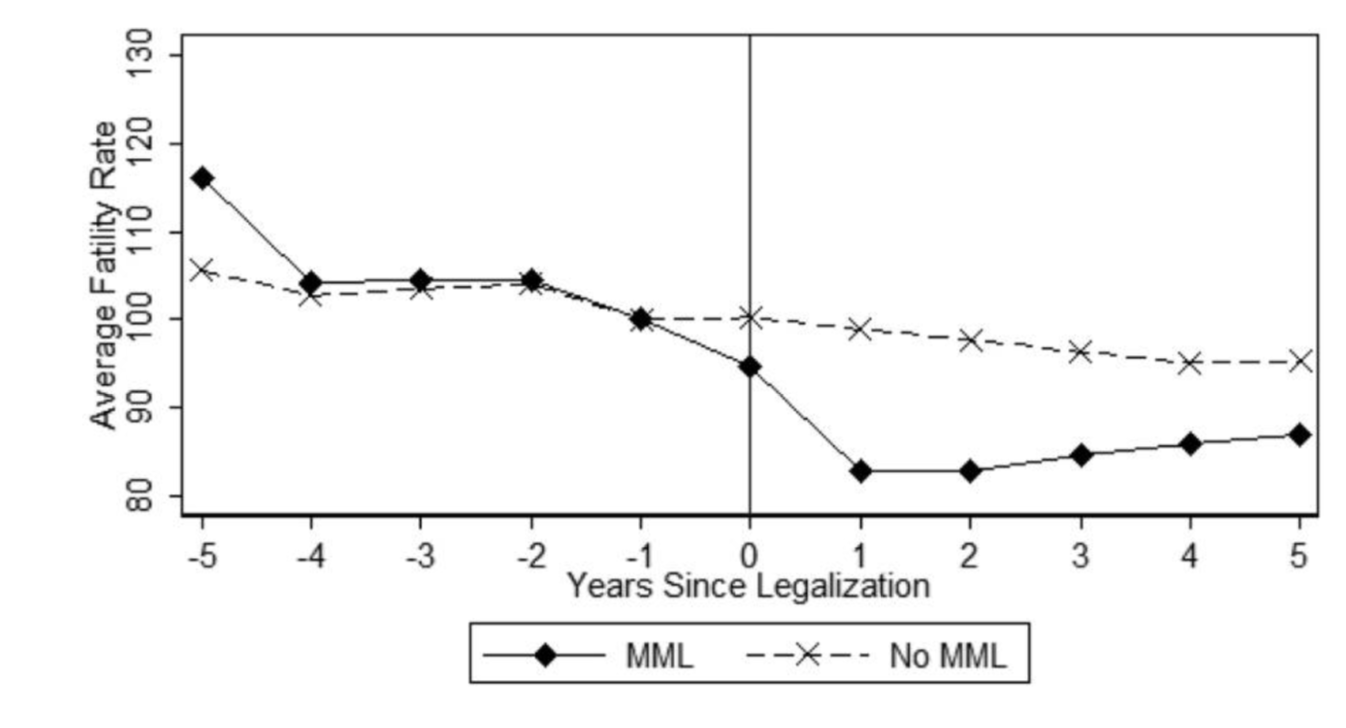
\includegraphics[width=0.62\textwidth,height=0.62\textheight,keepaspectratio]{figures/mml_eventstudy.png}
\end{center}
\vspace{-0.2em}
\begin{center}
\small\color{warmgray}\itshape
Anderson et al.\ (2013): raw traffic-fatality rates for treated states (re-centered to treatment date) vs.\ controls. The classic dynamic-effects display.
\end{center}
\end{frame}

%% ---------- L6-F2: The classic event-study spec ----------
\begin{frame}{The classic dynamic-TWFE event-study spec}
\vspace{0.4em}
Researchers want to plot pre-treatment placebo coefficients and post-treatment dynamic effects. \;The standard regression:
\vspace{0.4em}
\begin{center}
$Y_{i,t} \;=\; \alpha_i \;+\; \delta_t \;+\; \displaystyle\sum_{g \in G} \mu_g\,\mathbf{1}\{t - E_i \in g\} \;+\; \varepsilon_{i,t}$
\end{center}
\vspace{0.4em}
\begin{itemize}\small
  \item $E_i$ is unit $i$'s treatment date. \;$t - E_i$ is event time (relative-to-treatment).
  \item $G$ is the set of event-time bins (leads and lags) included.
  \item Coefficient $\mu_g$ is supposed to be the average treatment effect at event-time bin $g$.
\end{itemize}
\vspace{0.4em}
\highlight{Bacon told us static TWFE is biased.} \;Sun \& Abraham (2021) ask: \textit{what about the dynamic version?}
\end{frame}

%% ---------- L6-F3: SA's proposition ----------
\begin{frame}{Each lead and lag picks up treatment effects from \textit{other} leads and lags}
\vspace{0.4em}
Write $\text{ATT}_{e,l}$ for the treatment effect on cohort $e$ at $l$ years from its treatment date.

\vspace{0.4em}
Even under parallel trends and no anticipation, the TWFE coefficient on event-time bin $g$ is:

\vspace{0.3em}
\begin{align*}
\mu_g \;=\; & \underbrace{\textstyle\sum_{l \in g} \sum_e w^g_{e,l}\, \text{ATT}_{e,l}}_{\text{the target (own bin)}} \\[0.2em]
            & + \underbrace{\textstyle\sum_{g' \neq g} \sum_{l' \in g'} \sum_e w^g_{e,l'}\, \text{ATT}_{e,l'}}_{\text{leakage from \textit{other} included bins}} \\[0.2em]
            & + \underbrace{\textstyle\sum_{l' \in g^{\text{excl}}} \sum_e w^g_{e,l'}\, \text{ATT}_{e,l'}}_{\text{leakage from \textit{excluded} bins}}
\end{align*}
\vspace{0.1em}
\highlight{The cross-bin weights sum to zero --- but only cancel when treatment effects are identical across cohorts.} \;Once they're heterogeneous, the leakage doesn't cancel.
\end{frame}

%% ---------- L6-F4: What this means in practice ----------
\begin{frame}{The disturbing corollary: pre-period $\mu_g$ can be nonzero even when PT holds}
\vspace{0.5em}
Under PT $+$ no anticipation but \textit{not} homogeneity:
\vspace{0.5em}
\begin{itemize}\small
  \item A pre-period lead $\mu_{-2}$ should be zero if pre-trends are truly parallel.
  \item In TWFE it isn't --- it picks up post-treatment effects from \textit{other} cohorts through the cross-bin weights.
  \item So a ``failed placebo'' may just be the cross-bin leakage.
  \item And a ``passing placebo'' may just be cancellation, not evidence of parallel trends.
\end{itemize}
\vspace{0.5em}
\textbf{Lesson:} \;Don't drop excluded bins arbitrarily. \;Lagged effects contaminate through the excluded bins.

\vspace{0.4em}
\meta{Same disease as Bacon's static decomposition, but applied to leads and lags --- so it affects the entire \textit{plot} you're showing the audience.}
\end{frame}

%% ---------- L6-F5: SA's fix - the IW estimator ----------
\begin{frame}{SA's fix: the interaction-weighted estimator (3 steps)}
\vspace{0.4em}
\begin{enumerate}\small
  \item \textbf{Estimate each $\widehat{\delta}_{e,l}$ separately.} \;A saturated regression with cohort $\times$ event-time interactions, using the never-treated (or last-treated) as control:
  \vspace{0.1em}
  \begin{center}\scriptsize
  $Y_{i,t} \;=\; \alpha_i \;+\; \lambda_t \;+\; \displaystyle\sum_{e \notin C} \sum_{l \neq -1} \delta_{e,l}\big[\mathbf{1}\{E_i = e\} \cdot D^l_{i,t}\big] \;+\; \varepsilon_{i,t}$
  \end{center}
  \item \textbf{Estimate cohort shares} in the relevant periods: \;$\widehat{\Pr}(E_i = e \mid E_i \in [-l, T-l])$.
  \item \textbf{Aggregate} the $\widehat{\delta}_{e,l}$ using the cohort shares as weights.
\end{enumerate}
\vspace{0.5em}
\textbf{Same logic as CS.} \;Estimate cohort-event-time cells first; aggregate after. \;\highlight{Forward-engineer the parameter.}
\vspace{0.4em}
\meta{Software: \texttt{eventstudyinteract} (Stata, SSC); \texttt{fixest::sunab} (R).}
\end{frame}

%% ---------- L6-F6: TWFE vs SA, side by side ----------
\begin{frame}{TWFE event study vs.\ SA, side by side}
\begin{center}
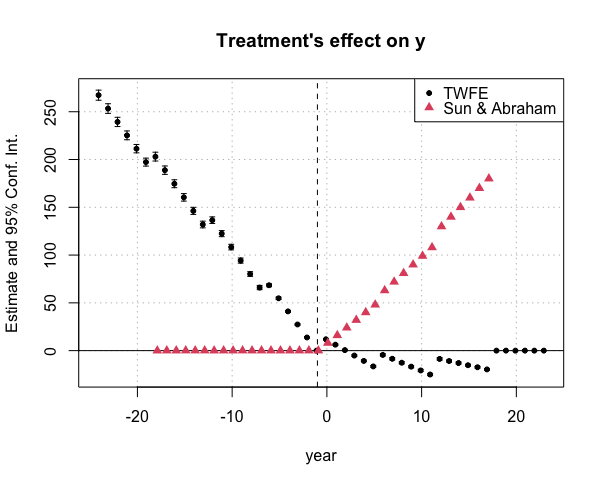
\includegraphics[width=0.78\textwidth,height=0.68\textheight,keepaspectratio]{figures/twfe_vs_sa_event.png}
\end{center}
\vspace{-0.3em}
\begin{center}
\small\color{warmgray}\itshape
TWFE leads slope downward pre-treatment --- the cross-bin contamination. \;SA's pre-period sits at zero; lags trace the dynamic profile.
\end{center}
\end{frame}

%% =====================================================================
%%                                LESSON 7
%% =====================================================================
\remixsection{7.\ de Chaisemartin \& D'Haultf{\oe}uille \\[0.3em] {\normalsize\normalfont Negative weights on \textit{unit-level} effects, plus the on-off case}}

%% ---------- L7-F1: What dCdH adds ----------
\begin{frame}{dCdH (2020) adds three things to the staggered toolkit}
\vspace{0.5em}
\begin{enumerate}\small
  \item \textbf{A different decomposition.} \;Bacon decomposed TWFE into 2$\times$2 building blocks with \textit{positive} weights. \;dCdH decomposes TWFE into \textit{unit-level} treatment effects --- where weights can be \highlight{negative}.
  \vspace{0.3em}
  \item \textbf{The on-off case.} \;CS and SA assume irreversible treatment. \;dCdH handles units that switch into and out of treatment (think: a state policy that was repealed). Roe v.\ Wade adopted in 1973, overturned in 2022.
  \vspace{0.3em}
  \item \textbf{A diagnostic.} \;Run the TWFE you were going to run, then count the \textit{share of unit-period treatment effects} that receive negative weights. Report the sign-flip threshold.
\end{enumerate}
\end{frame}

%% ---------- L7-F2: The decomposition ----------
\begin{frame}{The dCdH decomposition: weights on \textit{cell-level} treatment effects}
\vspace{0.4em}
Let $\Delta_{g,t}$ be the average treatment effect for group $g$ in period $t$ --- one number per treated cell of the panel. \;Under parallel trends and no anticipation:
\vspace{0.3em}
\begin{block}{Theorem 1 (dCdH 2020)}
\centering
$\beta_{\text{fe}} \;=\; \mathbb{E}\!\left[\displaystyle\sum_{(g,t):\,D_{g,t}=1} \tfrac{N_{g,t}}{N_1}\, w_{g,t}\, \Delta_{g,t}\right], \quad \displaystyle\sum_{(g,t)}\tfrac{N_{g,t}}{N_1}w_{g,t} = 1, \quad w_{g,t} \text{ \textbf{can be negative}}.$
\end{block}
\vspace{0.4em}
\begin{itemize}\small
  \item The weights $w_{g,t}$ are built from the residuals of regressing $D_{g,t}$ on group and time fixed effects.
  \item Bacon decomposes the \textit{estimator} into 2$\times$2 building blocks (always positive). \;dCdH decompose the \textit{estimand} into cell-level effects (\highlight{may be negative}).
  \item And dCdH applies to \textit{any} TWFE design, not just staggered.
\end{itemize}
\end{frame}

%% ---------- L7-F3: Why negative weights are dangerous ----------
\begin{frame}{Negative weights break the ``no sign-flip property''}
\vspace{0.5em}
\textbf{Thought experiment.} \;Suppose every treated cell gained from the treatment ($\Delta_{g,t} > 0$ for all $(g,t)$).
\vspace{0.4em}
\begin{itemize}\small
  \item If all $w_{g,t} > 0$: TWFE is a positive weighted average of positive effects. \;Sign matches.
  \item If some $w_{g,t} < 0$: nothing prevents TWFE from being \highlight{negative} --- even though every cell gained.
\end{itemize}
\vspace{0.6em}
\textbf{This is what we saw in baker.do.} \;Truth $+82$, TWFE $-6.69$. Some cells got large negative weights; they swamped the positive-weight contributions.
\vspace{0.5em}
\meta{Pre-dCdH, ``OLS is a weighted average'' was reassuring. dCdH made it disturbing.}
\end{frame}

%% ---------- L7-F4: When does it bite ----------
\begin{frame}{When the negative weights bite (and when they don't)}
\vspace{0.4em}
\textbf{Run two diagnostics on your data before publishing:}
\vspace{0.4em}
\begin{enumerate}\small
  \item \textbf{The share of treated cells with negative weight.} \;If a meaningful fraction of cells gets a minus sign, your headline is built on those cancellations.
  \item \textbf{The smallest amount of heterogeneity in $\Delta_{g,t}$ that could flip the sign of TWFE.} \;If small, your sign is fragile. If large, your sign is robust.
\end{enumerate}
\vspace{0.5em}
\textbf{Rules of thumb:}
\begin{itemize}\small
  \item A big never-treated group helps: fewer negative weights, smaller magnitudes.
  \item Treatment dates packed close together: also fewer.
  \item A long panel with a few early-treated cohorts: the worst case.
\end{itemize}
\vspace{0.4em}
\meta{Software: \texttt{twowayfeweights} (Stata SSC); R via \texttt{TwoWayFEWeights}. \;Both numbers come out on your specific dataset.}
\end{frame}

%% ---------- L7-F5: The on-off case ----------
\begin{frame}{The on-off case: \texttt{did\_multiplegt} for switching treatment}
\vspace{0.5em}
Suppose treatment can switch on \textit{and} off (Roe v.\ Wade 1973 $\to$ Dobbs 2022; minimum-wage rollbacks; tax cuts that sunset).
\vspace{0.4em}
\begin{itemize}\small
  \item CS and SA both assume \highlight{irreversible} treatment --- they cannot estimate effects in this setting.
  \item dCdH propose a different estimator built on \textit{instantaneous} effects between adjacent periods, comparing units that just switched against units whose treatment status is unchanged.
  \item Equivalent to CS \&\ SA when treatment is irreversible (with their particular weighting), but \textit{also} handles the on-off case.
\end{itemize}
\vspace{0.5em}
\meta{Software: \texttt{did\_multiplegt} (Stata); the \texttt{DIDmultiplegt} R package.}
\end{frame}

%% ---------- L7-F6: The weighting lesson ----------
\begin{frame}{The unifying lesson across Bacon, SA, and dCdH}
\begin{block}{What makes weights ``good''}
\centering
The economic question is: \textit{what parameter do you want?} \\[0.2em]
OLS doesn't ask. OLS picks weights from the residual variance of $D$.
\end{block}
\vspace{0.5em}
\begin{itemize}\small
  \item Bacon: TWFE = weighted average of 2$\times$2s. Weights positive, driven by treatment-status variance.
  \item SA: $\mu_g$ = weighted average of treatment effects across cohorts and event-times. Cross-bin leakage.
  \item dCdH: TWFE = weighted average of cell-level treatment effects $\Delta_{g,t}$. \highlight{Weights can be negative.}
\end{itemize}
\vspace{0.5em}
\textbf{All three say the same thing:} if you let OLS pick the weights, you've let it pick your economic question. \;Forward-engineer instead.
\end{frame}

%% =====================================================================
%%                                LESSON 8
%% =====================================================================
\remixsection{8.\ Borusyak-Jaravel-Spiess imputation \\[0.3em] {\normalsize\normalfont The Heckman-Ichimura-Todd move, lifted to fixed effects}}

%% ---------- L8-F1: All causal inference is imputation ----------
\begin{frame}{All causal inference is imputation}
\vspace{0.6em}
\begin{block}{Imbens \& Rubin (2015), \textit{Causal Inference}}
\centering
\itshape
``At some level, all methods for causal inference can be viewed as imputation methods, although some more explicitly than others.''
\end{block}

\vspace{0.7em}
\textbf{What's the missing thing?} \;Always $Y^0$ for the treated. \;What we never observe.

\vspace{0.4em}
\textbf{What's the estimator?} \;A model for $Y^0$ fit on the people who reveal it (the untreated), then plugged in for the treated.

\vspace{0.5em}
\highlight{You already saw one today.} \;Yesterday afternoon's OR-DiD was imputation. \;BJS is the same trick, with a different model.
\end{frame}

%% ---------- L8-F2: Recap HIT/OR-DiD ----------
\begin{frame}{Yesterday's HIT / OR-DiD recipe (recap)}
\vspace{0.5em}
\textbf{Heckman, Ichimura, Todd (1997).} \;The conditional-PT version of imputation:
\vspace{0.5em}
\begin{enumerate}\small
  \item \textbf{Fit the model} of the untreated trend on $X$, using only $D=0$:
  \begin{center}\small
  $\widehat{\mu}_0(X) \;=\; \widehat{\mathbb{E}}[\Delta Y \mid D{=}0,\, X]$
  \end{center}
  \item \textbf{Impute} each treated unit's counterfactual trend $\widehat{\mu}_0(X_i)$.
  \item \textbf{Average} the residual on the treated:
  \begin{center}\small
  $\widehat{\delta}_{\text{OR}} \;=\; \dfrac{1}{N_1}\displaystyle\sum_{i:D_i=1}\big(\Delta Y_i - \widehat{\mu}_0(X_i)\big)$
  \end{center}
\end{enumerate}
\vspace{0.5em}
\textbf{The counterfactual model is on \boldmath$\Delta Y$, indexed by \boldmath$X$.}
\end{frame}

%% ---------- L8-F3: The BJS recipe ----------
\begin{frame}{The BJS (2024) recipe, side-by-side}
\vspace{0.5em}
\textbf{Borusyak, Jaravel, Spiess (2024).} \;Same imputation logic, but the counterfactual model is on \textit{levels} $Y(0)$ indexed by \textit{fixed effects}:
\vspace{0.5em}
\begin{enumerate}\small
  \item \textbf{Fit the model} of untreated $Y(0)$ on unit FE $+$ time FE (and any pre-treatment $X$), using only $D=0$ observations:
  \begin{center}\small
  $Y(0)_{it} \;=\; \alpha_i \;+\; \lambda_t \;+\; X'_{it}\delta \;+\; \varepsilon_{it}$
  \end{center}
  \item \textbf{Impute} the counterfactual for each treated $(i,t)$: \;$\widehat{Y}^0_{it} \;=\; \widehat{\alpha}_i + \widehat{\lambda}_t + X'_{it}\widehat{\delta}$.
  \item \textbf{Average} the residual on the treated unit-periods:
  \begin{center}\small
  $\widehat{\tau}_{it} \;=\; Y^1_{it} - \widehat{Y}^0_{it}, \qquad \widehat{\delta}_W \;=\; \displaystyle\sum_{(i,t)\in\Omega_1} w_{it}\,\widehat{\tau}_{it}$
  \end{center}
\end{enumerate}
\vspace{0.4em}
\highlight{Same three moves as HIT.} \;Only the counterfactual model differs.
\end{frame}

%% ---------- L8-F4: Why it works (no forbidden contrast) ----------
\begin{frame}{Why BJS avoids the forbidden contrast}
\vspace{0.5em}
The fixed-effects regression in Step 1 is fit on \highlight{untreated observations only.}

\vspace{0.5em}
\begin{itemize}\small
  \item No treated observation enters the model that predicts $Y(0)$.
  \item Already-treated units contribute their pre-treatment periods only (those are still untreated).
  \item The fixed effects propagate across time, so $\widehat{\alpha}_i$ for unit $i$ can still be estimated even if $i$ is eventually treated --- using $i$'s own pre-treatment observations.
\end{itemize}

\vspace{0.6em}
\textbf{Compare to TWFE.} \;TWFE fits $\delta$ \textit{and} the fixed effects on \textit{all} observations simultaneously --- so a treated unit's post-period influences the estimated FE, which feeds back into the residual that defines $\widehat{\delta}$. That's the forbidden-contrast channel.

\vspace{0.5em}
\highlight{BJS just refuses to let that happen.} \;Same model class, different fitting sample.
\end{frame}

%% ---------- L8-F5: BJS comparison plot ----------
\begin{frame}{BJS compared with TWFE, CS, SA on the same DGP}
\begin{center}
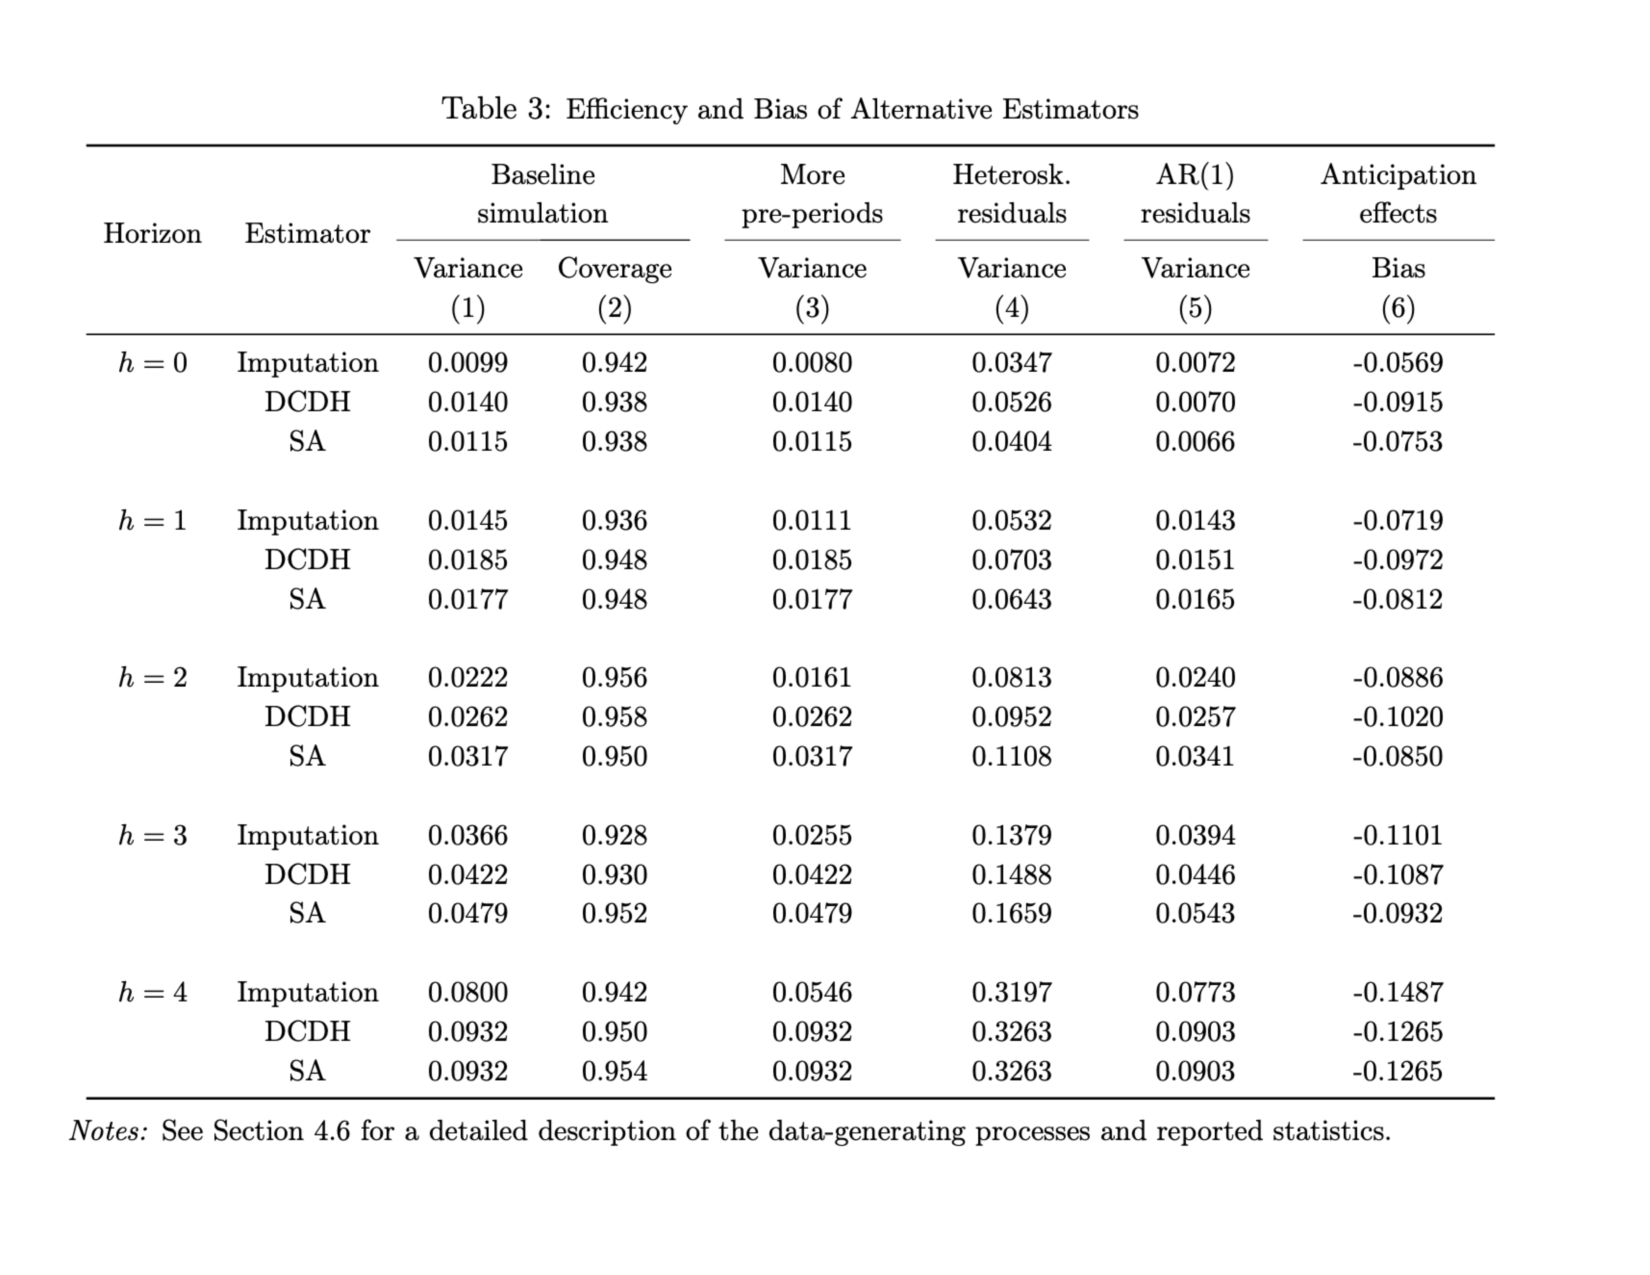
\includegraphics[width=0.74\textwidth,height=0.68\textheight,keepaspectratio]{figures/bjs_comparison.pdf}
\end{center}
\vspace{-0.3em}
\begin{center}
\small\color{warmgray}\itshape
TWFE event-study: biased pre-period leads, attenuated lags. \;CS, SA, BJS all recover the dynamic profile. \;Three different counterfactual models, same answer.
\end{center}
\end{frame}

%% ---------- L8-F6: When to use which ----------
\begin{frame}{When BJS, when CS, when SA, when dCdH?}
\vspace{0.4em}
\begin{itemize}\small
  \item \textbf{CS (DR).} \;You want $\text{ATT}(g,t)$ building blocks. \;You have covariates that matter for conditional PT. \;\highlight{First choice when standard staggered.}
  \item \textbf{SA.} \;You specifically want an event-study plot. \;Equivalent to CS with never-treated; gives closed-form SEs.
  \item \textbf{BJS.} \;You want a single $\widehat{\tau}_{it}$ for every treated unit-period --- maximum flexibility, can compute any aggregate. \;Comfortable assuming the parametric Y(0) model.
  \item \textbf{dCdH.} \;Your treatment switches \textit{on and off}. \;CS, SA, BJS all assume irreversibility; dCdH does not.
\end{itemize}
\vspace{0.4em}
\meta{Practitioner's guide framing: all four are forward-engineered estimators. Pick the one that matches the parameter you want and the assumptions you can defend.}
\end{frame}

%% =====================================================================
%%                                LESSON 9
%% =====================================================================
\remixsection{9.\ Honest DiD \\[0.3em] {\normalsize\normalfont You can't test parallel trends. You can bound the violation.}}

%% ---------- L9-F1: PT is not testable ----------
\begin{frame}{Parallel trends is not testable. Pretests are not the same assumption.}
\vspace{0.4em}
\textbf{The standard ritual.} \;Show that pre-period coefficients are statistically indistinguishable from zero. \;Conclude: ``parallel trends holds.''
\vspace{0.5em}

\textbf{Roth (2022) showed this is a mistake.}
\begin{itemize}\small
  \item Pre-trends measure differences in the \textit{wrong} periods --- they test whether trends were parallel \textit{before} treatment, not whether they'd be parallel \textit{after} in its absence.
  \item Pre-tests are typically \highlight{low-powered}: failing to reject ``$\beta_{\text{pre}} = 0$'' is consistent with non-trivial violation.
  \item Conditioning on the pretest passing \textit{distorts} the post-period estimator (selection on the pretest outcome).
\end{itemize}
\vspace{0.4em}
\highlight{You cannot test PT. \;What you can do: bound the plausible violation.}
\end{frame}

%% ---------- L9-F2: Rambachan-Roth reframing ----------
\begin{frame}{Rambachan \& Roth (2023): bound the violation, get partial-ID bounds}
\vspace{0.5em}
\textbf{The reframe.} \;Take the post-period PT violation $\delta_t = \mathbb{E}[Y^0_t - Y^0_{t-1} \mid D{=}1] - \mathbb{E}[Y^0_t - Y^0_{t-1} \mid D{=}0]$ as an unknown nuisance.

\vspace{0.5em}
\begin{enumerate}\small
  \item Pick a \textit{class} of plausible $\delta_t$ paths.
  \item For each path in that class, the ATT is point-identified.
  \item The union over the class gives a \highlight{partial-identification interval} for the ATT.
\end{enumerate}

\vspace{0.5em}
\textbf{The output isn't a point estimate.} \;It's a \textit{robust confidence set}: ``if the violation belongs to this class, the ATT lies in this interval.''

\vspace{0.4em}
\meta{Software: \texttt{HonestDiD} in R; \texttt{honestdid} in Stata (M.\ C{\'a}ceres Bravo). \;Plugs into the output of CS, SA, or BJS.}
\end{frame}

%% ---------- L9-F3: Two restriction classes ----------
\begin{frame}{Two restriction classes: smoothness ($M$) and relative magnitudes ($\bar M$)}
\vspace{0.4em}
\textbf{Smoothness ($M$-class).} \;The violation can't accelerate too fast:
\begin{center}\small
$|\delta_{t+1} - \delta_t| \;\leq\; M \quad\text{for all } t.$
\end{center}
``Trajectory of any unobserved violation is at most $M$ units off a line.'' \;Larger $M$ $\Rightarrow$ more flexibility $\Rightarrow$ wider bounds. \;$M=0$ pins down linear extrapolation.

\vspace{0.6em}
\textbf{Relative magnitudes ($\bar M$-class).} \;Post-period violation $\leq \bar M$ times the largest pre-period observed difference:
\begin{center}\small
$|\delta_{\text{post}}| \;\leq\; \bar M \cdot \max_{\text{pre}}|\widehat{\delta}_{\text{pre}}|.$
\end{center}
``If the pre-trend looks small, the post-trend can't be much bigger.'' \;Common values $\bar M \in \{0.5,\, 1,\, 2\}$.

\vspace{0.3em}
\highlight{Pick the class that matches what you'd defend at the seminar.}
\end{frame}

%% ---------- L9-F4: The breakdown value ----------
\begin{frame}{The breakdown value: how much PT violation would erase your result?}
\vspace{0.4em}
For each $M$ (or $\bar M$), Rambachan-Roth give you a confidence set $\mathcal{C}(M)$ for the ATT.
\vspace{0.5em}
\begin{block}{Breakdown value}
\centering
$M^{\text{break}} \;=\; \min\{\, M \;:\; 0 \in \mathcal{C}(M)\,\}.$
\end{block}
\vspace{0.5em}
\textbf{Read it.} \;``If parallel trends is allowed to deviate by more than $M^{\text{break}}$ per period, my significant result could vanish.''

\vspace{0.5em}
\begin{itemize}\small
  \item Large breakdown value $\Rightarrow$ result is robust to plausible violations.
  \item Small breakdown value $\Rightarrow$ result is fragile; even tiny violations break significance.
  \item Reported \textit{alongside} the headline, not in place of it.
\end{itemize}
\vspace{0.3em}
\meta{This is the diagnostic you'll compute on the Brazil mental-health-reform application in the lab.}
\end{frame}

%% =====================================================================
%%                                LESSON 10
%% =====================================================================
\remixsection{10.\ Synthesis \\[0.3em] {\normalsize\normalfont What's the same, what's different, what to do tomorrow morning}}

%% ---------- L6-F1: The afternoon-morning thread ----------
\begin{frame}{Yesterday afternoon plus this morning $=$ one workflow}
\vspace{0.5em}
\begin{itemize}
  \item \textbf{Yesterday (covariates).} \;Conditional PT $\Rightarrow$ DR-DiD. \;Two chances to be right (OR model or pscore model).
  \vspace{0.3em}
  \item \textbf{This morning (staggered).} \;ATT$(g,t)$ building blocks, estimated cell-by-cell, then aggregated.
  \vspace{0.3em}
  \item \textbf{The combination.} \;Each ATT$(g,t)$ \textit{is} a 2$\times$2 problem. \;The recommended way to estimate it is DR-DiD with whatever $X$ you need for conditional PT. \;Then aggregate.
\end{itemize}

\vspace{0.7em}
\begin{block}{One sentence}
\centering
\highlight{Forward-engineer the target, estimate the cells with DR, aggregate with non-negative weights.}
\end{block}
\end{frame}

%% ---------- L6-F2: When to use TWFE ----------
\begin{frame}{When to use TWFE in staggered settings}
\vspace{0.6em}
\begin{center}
\Huge\bfseries\color{harvardcrimson} Basically never.
\end{center}

\vspace{0.6em}
\begin{itemize}\small
  \item TWFE = ATT only when (a) treatment effects are homogeneous across cohorts, AND (b) treatment effects don't change over time within a cohort.
  \item Both fail in almost every applied setting.
  \item Even when they hold, the variance weights are still strange (depend on panel length).
  \item \textbf{If you must report it, also report CS, SA, BJS, or dCdH --- and the dCdH negative-weight diagnostic. Explain the differences.}
\end{itemize}

\vspace{0.5em}
\meta{Baker, Callaway, Cunningham, Goodman-Bacon, Sant'Anna (2025): ``Do not use TWFE.''}
\end{frame}

%% ---------- L6-F3: A student asks ----------
\begin{frame}{A student asks: ``But what about my paper from last year that used TWFE?''}
\vspace{0.4em}
A reasonable thing to do, in order:

\vspace{0.5em}
\begin{enumerate}\small
  \item \textbf{Run the Bacon decomposition} (\texttt{ddtiming}; \texttt{bacondecomp} in R). \;See whether the forbidden 2$\times$2s carry weight.
  \item \textbf{Run the dCdH diagnostic} (\texttt{twowayfeweights}). \;Sizeable negative-weight share $\Rightarrow$ headline is suspect.
  \item \textbf{Re-estimate with CS, SA, or BJS.} \;Compare the new headline to TWFE.
  \item \textbf{If they disagree:} \;the difference \textit{is} the $-\Delta\text{ATT}$ / VWPT / negative-weight contamination. Trust the design-based estimator.
  \item \textbf{If they agree:} \;in your setting, dynamics and heterogeneity didn't bite. \;Report both, explain.
\end{enumerate}
\meta{Goodman-Bacon, Sant'Anna, Whitten (2026) gives a refined re-analysis framework for pre-trends-parallel settings.}
\end{frame}

%% ---------- Lab: Brazil mental-health reform ----------
\begin{frame}{Lab: the 9-step checklist on Dias \&\ Fontes (2024)}
\vspace{0.2em}
\textbf{The paper.} \;CAPS mental-health centers rolling out across Brazilian municipalities, 2002--2016. \;Outcome: homicide rate.
\vspace{0.4em}
\begin{enumerate}\scriptsize
  \item Decide on the target parameter (write down what you want, then defend it).
  \item Cohort count table. \;Identify never-treated, always-treated. \;Drop the 2002 cohort and say why.
  \item Plot the treatment rollout (calendar grid in grayscale).
  \item Plot the raw outcome by cohort. \;What do you see before estimation?
  \item Covariate balance table (normalized differences, 2002 baseline).
  \item Run TWFE first as a \textit{diagnostic} (don't interpret causally yet).
  \item Bacon decomposition \&\ dCdH negative-weight diagnostic.
  \item CS with DR-DiD: simple, group, calendar, event aggregations.
  \item Honest DiD: $\bar M$-bounds and breakdown value.
\end{enumerate}
\vspace{0.3em}
\meta{Walkthrough: \texttt{zurich/labs/Brazil/README.md}. \;Reference code: \texttt{labs/Brazil/code/brazil.do} and \texttt{brazil.R}. \;Data on Scott's GitHub: \texttt{mixtape/brazil.dta}.}
\end{frame}

%% ---------- Tomorrow ----------
\begin{frame}{Tomorrow afternoon}
\vspace{0.5em}
\begin{itemize}
  \item \textbf{Honest event-studies.} \;Roth (2022) on conditioning on pretest passes. \;Rambachan \& Roth (2023) partial-identification bounds.
  \item \textbf{Continuous and multi-valued treatment.} \;Dose-specific ATT, average causal response (Callaway, Goodman-Bacon, Sant'Anna 2024).
  \item \textbf{Goodman-Bacon, Sant'Anna, Whitten (2026)} --- a refined re-analysis framework for pre-trends-parallel settings.
  \item \textbf{Two-stage DiD} (Gardner 2021) --- the GMM cousin of BJS, with the same forward-engineered architecture.
\end{itemize}

\vspace{0.7em}
\begin{center}\large
Reading for tonight: \;\textit{Baker, Callaway, Cunningham, Goodman-Bacon, Sant'Anna (2025)}\\
\textit{``Difference-in-Differences Designs: A Practitioner's Guide.''}
\end{center}
\end{frame}

%% ---------- Final ----------
\begin{frame}[plain]
\centering
\vspace{2.5em}
{\Huge\bfseries\color{forest} Forward-engineer.}\\[1.5em]
{\Large\itshape\color{charcoal} Start with what you want to estimate.\\Match the estimator to the assumption.\\Aggregate at the end, not the start.}\\[2em]
\rule{0.4\textwidth}{0.6pt}\\[0.8em]
{\small\color{warmgray} Scott Cunningham \textperiodcentered\ University of Zurich \textperiodcentered\ May 13, 2026}
\end{frame}

\end{document}
